%&pdflatex
%% filename: amsart-template.tex, version: 1.1
\documentclass{amsart}
\usepackage{hyperref} % for hyperlinks
\usepackage{inputenc} % for french
\usepackage{listings} % for code
\usepackage{graphicx}
\usepackage{booktabs} % For \toprule, \midrule and \bottomrule
%\usepackage{siunitx} % Formats the units and values
%\usepackage{pgfplotstable} % Generates table from .csv
\usepackage{csvsimple}

\newtheorem{theorem}{Theorem}[section]
\newtheorem{lemma}[theorem]{Lemma}

\theoremstyle{definition}
\newtheorem{definition}[theorem]{Definition}
\newtheorem{example}[theorem]{Example}
\newtheorem{xca}[theorem]{Exercise}

\theoremstyle{remark}
\newtheorem{remark}[theorem]{Remark}

\numberwithin{equation}{section}

\lstset{
    language=Python,
    frame=lines,
    label={lst:code_direct},
    basicstyle=\footnotesize,
    breaklines=true
}

%sisetup{
%  round-mode          = places, % Rounds numbers
%  round-precision     = 2, % to 2 places
%}


\graphicspath{ {./} }

\setlength{\parindent}{0pt} % turn off auto-indent

\begin{document}

\title{Assignment 1: Implementation of Multi Layer Perceptrons [IFT6135]}

\author{Joseph D. Viviano, Jonathan Guymont, Marzieh Mehdizadeh}
\address{Universit\'e de Montr\'eal}
\curraddr{}
\email{joseph@viviano.ca, jonathan.guymont@.com, marzieh.mehdizadeh@gmail.com}
\thanks{}

\date{Feburary 2018}

\maketitle

\section{MLPs on MNIST}

The initial model build contained the following parameters for the layers:

$h_0$ = 784 units (input layer). \\
$h_1$ = 512 units (hidden layer 1). \\
$h_2$ = 512 units (hidden layer 2). \\
$h_3$ = 10 units (output layer, softmax). \\

This resulted in a model with 669,706 parameters (adding up all weight matrices
and biases): \\

$n = (512 \times 784) + (512) + (512 \times 512) + (512) + (10 \times 512) + (10)$ \\

Please see Appendix A for the implementation of the MLP. \\


\subsection{Initialization Schemes}

We compared training performance of the above MLP under three weight initialization
conditions: 1) where all weights are initialized to zeros, 2) where each weight
was sampled from a Normal distribution, and 3) where the initial weights were
sampled from a uniform distribution using the Glorot initialization scheme. \\

The above model was trained using ReLU nonlinearties, a learning rate of 0.01,
and a mini-batch size of 100 (shuffled), for 10 epochs. We used Stochastic
Gradient Descent (SGD) optimizer and cross entropy as our training criterion.
Please see the Appendix B for the implementation of the training loop. \\

\textbf{Figure 1} shows that the three initialization methods produced extremely
different behaviour in the loss function over epochs. \\

\begin{figure}[h]
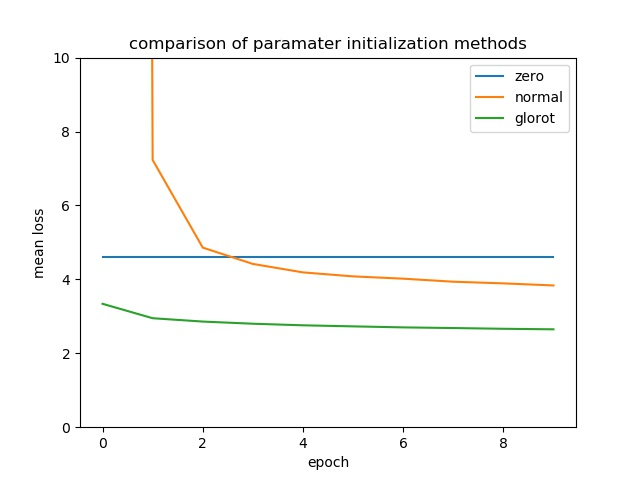
\includegraphics[width=100mm]{01_init_loss}
\caption{Comparison of initialization schemes.}
\label{Figure 1}
\end{figure}

Initialization using all zeros produced no learning, as the weights were unable
to break symmetry. Initialization using normally distributed weights produced
very large losses during the first few epochs before producing good results. This
is likely because the weight initialization used too many large values, producing
large gradients. Glorot initialization produced the best (lowest) losses
immediately and at the end of training. This is because the Glorot initialization
scheme aims to stabilize the activation variances and the back-propogated
gradiant variance, which leads to faster convergance. \\


\subsection{Learning Curves of Models of Differing Capacity}

In this section, we compared the learning curves of two models of differing
capacity. Both models were trained with a batch size of 100 (shuffled), learning
rate of 0.1, Glorot weight initialization, ReLU nonlinearities, and SGD with
cross entropy loss over 100 epochs. The small model had 266610 parameters: \\

$h_0$ = 784 units (input layer). \\
$h_1$ = 300 units (hidden layer 1). \\
$h_2$ = 100 units (hidden layer 2). \\
$h_3$ = 10 units (output layer, softmax). \\

\textbf{figure 2} shows the training and validation curves for this model: \\

\begin{figure}[h]
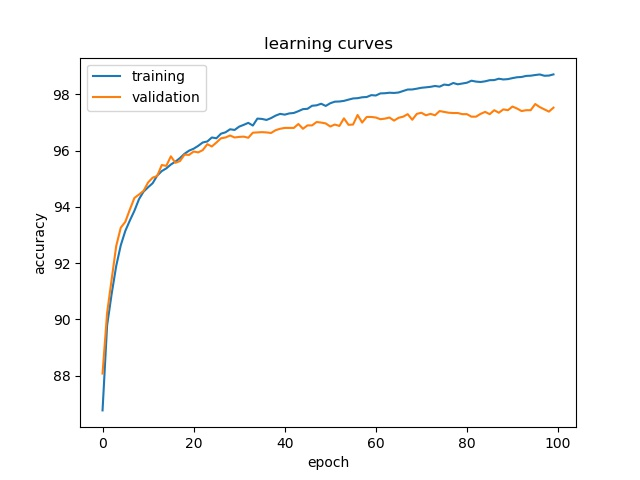
\includegraphics[width=100mm]{02_accuracy_266610_params}
\caption{Training curve of the small model.}
\label{Figure 2}
\end{figure}

The large model had 545810 parameters: \\

$h_0$ = 784 units (input layer). \\
$h_1$ = 500 units (hidden layer 1). \\
$h_2$ = 300 units (hidden layer 2). \\
$h_3$ = 10 units (output layer, softmax). \\

\textbf{figure 3} shows the training and validation curves for this model: \\

\begin{figure}[h]
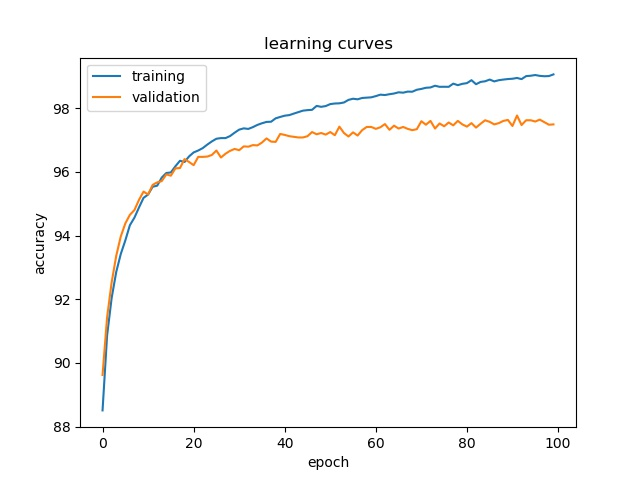
\includegraphics[width=100mm]{02_accuracy_545810_params}
\caption{Training curve of the large model.}
\label{Figure 3}
\end{figure}

As can be seen, the larger model confers no benefit on the validation set even
even though the training set accuracy is better. This is because the model with
larger capacity tends to fit the random noise in the training data, which
provides no information about the true relationship between the inputs and the
targets. Therefore, there is no improvement of the generalization error. When
the capacity of the model is high enough to cause the algorithms to memorize
random noise in the training set, we say that the model has high variance
because different training data are likely to produce a different model. \\


\subsection{Training Set Size, Generalization Gap, and Standard Error}

In this section, we compared the effect of training set size on the generalization
gap (difference between validation set accuracy and test set accuracy). We used
the large model from the previous section. All models were trained with a batch
size of 100 (shuffled), learning rate of 0.1, Glorot weight initialization, ReLU
nonlinearities, and SGD with cross entropy loss over 100 epochs. \\

We ran 5 tests, calculating the generalization gap when training with 1\%, 2\%,
5\%, 10\%, or 100\% of the training data. For each test, we ran 5 training
sessions using the above parameters. The results of these tests are shown below: \\

{\centering
\csvautotabular{03_gen_gap.csv}\par
}\\

As can be seen, with larger training set sizes, the generalization gap narrows
dramatically (from approximately 15\% difference in accuracy, down to a nearly
1\% difference in accuracy. Furthermore, the standard error of the mean across
the 5 trials also decreases, showing less variability in outcomes across the 5
training sessions when larger training set sizes are used. We conclude that
larger training set sizes produce more stable and accurate models with respect
to their generalization performance (i.e., test set performance). From a bias-
variance point of view, since the mean and the standard deviation of the
generalization gap are at their lowest when the training set size is the
highest, we could also say that increasing the size of the training set
decreases both bias and variance (assuming the added training set data truly
comes from the same distribution as the test and validation set data.).  \\


\section{MLPs on 20 Newsgroups}

\subsection{Preprocessing}

In this section we use the similar MLP as described before, but this time with
only one hidden layer of 100 units, and SGD used a momentum of 0.9, Glorot
initialization was used in all cases, as well as a batch size of 20. We compared
tf-idf and z-scoring preprocessing for text data with raw data, by analyzing
their training and test accuracies on the data using all three methods
(\textbf{figure 4}).  \\

\begin{figure}[h]
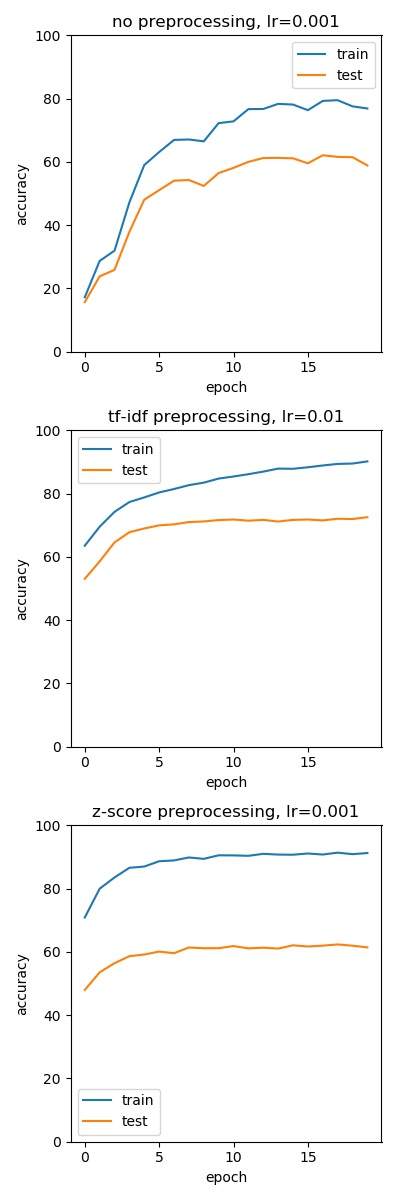
\includegraphics[width=50mm]{04_preproc}
\caption{Training curves for three preprocessing strategies.}
\label{Figure 4}
\end{figure}

First we observe that tf-idf preprocessing affords a learning rate one order of
magnitude greater than either using the raw data, or z-score normalized data. We
speculate that this is because the loss when analyzing tf-idf data is informed
more by high-information words. Both raw and z-score normalized text data give
high weight to common words like `and', `or', and `to', which carry no
information about document type since they are common across the entire corrupt.
Therefore the error gradient of models that include these low-information words
in prediction should be much steeper, as these low-information words would lead
to a lot of very bad predictions. In contrast, tf-idf downweights the
contribution of common words, and emphasizes regularly-appearing words in the
document, but not in the corpus, thereby focusing on features with high
information relevant to the task. \\

Second, if $\epsilon$ was zero during z-scoring, we could end up with NaNs in our
data set if the standard deviation of any word count was zero (i.e., that word
always occurs in documents the exact same number of times). This could be fixed
by replacing NaNs with some constant value, including zero. Another way to
minimize this problem would be to use something like min-max normalization (i.e,
scale all counts between 0-1), which is guaranteed not to divide your counts by
zero in any reasonable case. \\

Tf-idf's advantage, as explored above, is that it down-weights common words that
occur in all document types, allowing the model to focus on words unique to each
document type. This will result is a better document classifier. \\

\subsection{Variance in Training}

\textbf{Figure 5} shows the loss for the first 5000 minibatch updates for a model trained
on tf-idf preprocessed data, with a learning rate of 0.2 and a minibatch size of
either 1 or 100: \\

\begin{figure}[h]
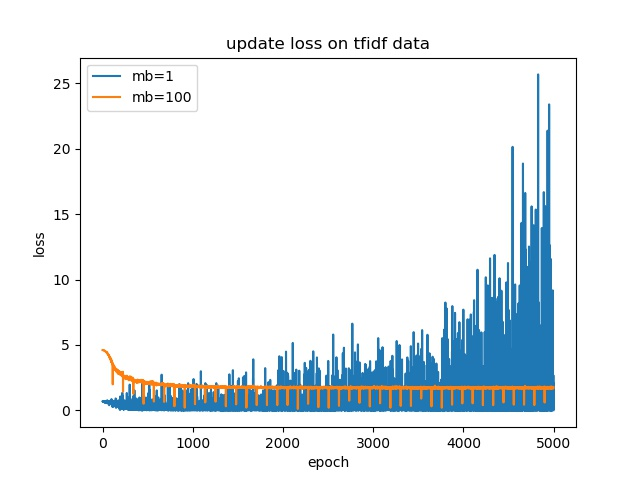
\includegraphics[width=100mm]{05_mbsize}
\caption{Minibatch size and the loss.}
\label{Figure 5}
\end{figure}

While both models have updates of the same magnitude, training performance is
very different. First, the gradient computed on single training examplesi (in
the minibatch=1 case) are likely to vary greatly from one another, so each
update is going to push the model in different directions. This results in the
high variance observed in this case. In contrast, the results seen in the
minibatch=100 case are effectively the average loss across 100 minibatch=1 cases,
which explains the lower variance. Furthermore, this plot is misleading. Since
the minibatch=100 loss plotted is the result of $100\times$ the training data of
the minibatch=1 loss, the end loss is much lower for the minibatch=100 case
because that case has trained on 100\times the training data. \\

We could reduce the variance of the minibatch=1 case simply by taking smaller
steps each update, that is, reducing the learning rate. Since each loss computed
on a single training sample is a noisy estimate of the population loss given the
model, the gradient is likely to be inaccurate. Therefore, large steps taken
dependent on these gradients are likely to be less productive than more
incremental steps.


\appendix
\section{MLP Model}

The MLP was implemented as a pytorch \texttt{Module} class. It accepts a list of
hidden layer sizes, allowing the user to specify an MLP of any length using 3
variables: \texttt{h0} = input size, \texttt{hn} = hidden layer sizes (as a
list), and \texttt{ho} = output size. \\

This class also contains an \texttt{initializer} method for initializing weights
and \texttt{count\_params} method for counting all model parameters).

\begin{lstlisting}[breaklines]

Class MnistMLP(torch.nn.Module):
    """MLP classifier for MNIST"""
    def __init__(self, h0, hn, ho):
        """
        h0 -- input size (flat)
        hn -- a list of all hidden layer sizes
        ho -- output size (number of classes; flat)
        """
        super(MnistMLP, self).__init__()

        # input --> hid1
        architecture = [torch.nn.Linear(h0, hn[0]), torch.nn.ReLU()]

        # hidden layers
        for i in range(1, len(hn)):
            architecture.append(torch.nn.Linear(hn[i-1], hn[i]))
            architecture.append(torch.nn.ReLU())

        # output
        architecture.append(torch.nn.Linear(hn[-1], ho))

        # use nn to define model
        self.mlp = torch.nn.Sequential(*architecture)
        self.clf = torch.nn.LogSoftmax(dim=0)

    def forward(self, X):
        return(self.clf(self.mlp(X).squeeze()))

    def initalizer(self, init_type='glorot'):
        """
        model     -- a pytorch sequential model
        init_type -- one of 'zero', 'normal', 'glorot'

        Takes in a model, initializes it to all-zero, normal distribution
        sampled, or glorot initialization. Golorot == xavier.
        """
        if init_type not in ['zero', 'normal', 'glorot']:
            raise Exception('init_type invalid]')

        for k, v in self.mlp.named_parameters():
            if k.endswith('weight'):
                if init_type == 'zero':
                    torch.nn.init.constant(v, 0)
                elif init_type == 'normal':
                    torch.nn.init.normal(v)
                elif init_type == 'glorot':
                    torch.nn.init.xavier_uniform(v, gain=calculate_gain('relu'))
                else:
                    raise Exception('invalid init_type')

    def count_params(self):
        """
        Returns a count of all parameters
        """
        param_count = 0
        for k, v in self.mlp.named_parameters():
            param_count += np.prod(np.array(v.size()))

        return(param_count)

\end{lstlisting}


\section{Training Loop}

The implementation of the training loop can be seen below, and is used throughout
the report: \\

\begin{lstlisting}[breaklines]

CUDA = torch.cuda.is_available()

def run_experiment(clf, lr, epochs, loaders, momentum=False, init_type='glorot'):

    if len(loaders) == 3:
        train, valid, test = loaders
    elif len(loaders) == 2:
        train, valid = loaders
        test = None
    else:
        raise Exception('loaders malformed')

    clf.initalizer(init_type=init_type)

    if CUDA:
        clf = clf.cuda()

    if momentum:
        optimizer = torch.optim.SGD(clf.parameters(), lr=lr, momentum=0.9)
    else:
        optimizer = torch.optim.SGD(clf.parameters(), lr=lr)

    #lossfn = torch.nn.CrossEntropyLoss() # don't use! B/C I specify LogSoftmax
    lossfn = torch.nn.NLLLoss()

    epoch_loss, valid_acc, train_acc = [], [], []
    best_valid_acc, gen_gap = 0, 0

    all_losses = []
    for ep in range(epochs):

        epoch_losses = []

        # training data
        for batch_idx, (X_train, y_train) in enumerate(train):

            if CUDA:
                X_train, y_train = X_train.cuda(), y_train.cuda()

            # initalize batch
            optimizer.zero_grad()
            X_train, y_train = Variable(X_train), Variable(y_train)

            # make predictions -- flatten each image (batchsize x pixels)
            train_pred = clf.forward(X_train.view(X_train.shape[0], -1))

            # calculate loss (cross entropy)
            loss = lossfn(train_pred, y_train)
            epoch_losses.append(loss.data[0])
            all_losses.append(loss.data[0])

            # calculate dloss/dx for all parameters that have requires_grad
            loss.backward()

            # update paramater values
            optimizer.step()

        # average loss for epoch
        epoch_loss.append(np.mean(epoch_losses))

        # validation accuracy for this epoch
        this_valid_acc = evaluate(clf, valid)
        valid_acc.append(this_valid_acc)

        # training accuracy for this epoch
        this_train_acc = evaluate(clf, train)
        train_acc.append(this_train_acc)

        # keep track of the best validation accuracy, generalization gap
        if this_valid_acc > best_valid_acc:
            best_valid_acc = this_valid_acc

            if test:
                this_test_acc = evaluate(clf, test)
                gen_gap = this_train_acc - this_test_acc

        # update every n epochs
        if (ep+1) % 5 == 0:
            curr_lr =  optimizer.state_dict()['param_groups'][0]['lr']
            print('+ [{:03d}] loss={:0.6f} acc={:0.2f}/{:0.2f} lr={:0.5f}'.format(
                ep+1, epoch_loss[-1], train_acc[-1], valid_acc[-1], curr_lr))

    results = {'clf': clf,
               'epoch_loss': epoch_loss,
               'all_loss': all_losses,
               'train_acc': train_acc,
               'valid_acc': valid_acc,
               'best_valid_acc': best_valid_acc,
               'gen_gap': gen_gap}

    return(results)

\end{lstlisting}

\end{document}
